\begin{Figure}
    \centering
    \footnotesize
		
		\psfrag{xp}[c][c] {$+$}
		\psfrag{xm}[c][c] {$-$}
		\psfrag{dta}[c][c] {$\delta x$}
		\psfrag{tuan}[c][c] {$\delta x$}
		
		\psfrag{mn}[c][c] {$\text{Solid electrolyte}$}
		\psfrag{gr}[c][c] {$\text{graphite}$}
		\psfrag{lico}[c][c] {$\text{Li-ion concentration}$}
		%\psfrag{sri}[c][c] {$\text{Solid electrolyte}$}
		\psfrag{a}[c][c] {$\text{(a)}$}
		\psfrag{b}[c][c] {$\text{(b)}$}
		
		
		
		%\includegraphics[scale=0.3]{batt.eps}te
    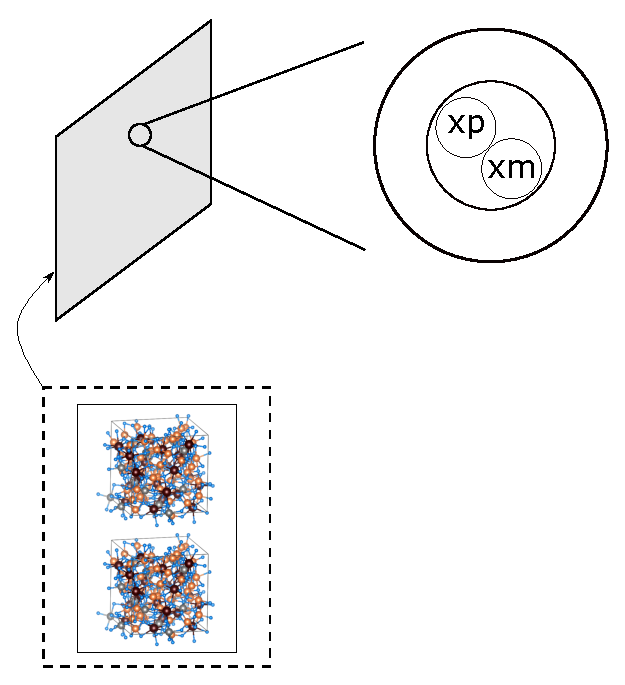
\includegraphics[width=0.4\textwidth]{polar.eps}
    %\caption{Swelling mechanism: Intercalation of Li-ion into graphite anode. (a) Concentration of Li-ion on graphite anode causes swelling phenomena to about $10\%$ of volume increase. (b) No concentration of Li-ion on graphite anode.}
    %\label{\LABEL}
		
\end{Figure}


